\chapter{Implementation}
Detailed description of all components and  functions here.  
\begin{csharpcode}
//UDPHandler Constructor 
public UDPHandler(String IP, Int32 Port, Int32 Timeout)
{
    ServerAddr = IPAddress.Parse(IP);
    EndPoint = new IPEndPoint(ServerAddr, Port);
    sock.ReceiveTimeout = Timeout;
    s = new UdpClient(IP, Port);
    
    EncryptionKeyDefault = "YiyM/f2zNq5GkVmiUMJ8qVACaPaBBo5AJRqkIH9cgd4=";
    EncryptionIVDefault = "tLafaj6+1YCiIIvbMO7iN/9QVLK1PPjRzARR9Fsh82c=";
}
\end{csharpcode}
PHP Code
\begin{phpcode}
<?php
class Payload
{
    public $Nth;
    public $outOfN;
    public $content;
    //konstruktor
    public function __construct($Nth, $outOfN, $content)
    {
        $this->Nth = $Nth;
        $this->outOfN = $outOfN;
        $this->content = $content;
    }
}
?>
\end{phpcode}

\section{Database design}
For this purposes a well defined database is a necessity. In this chapter we're going to learn how the proposed objects are represented, how relations between these objects are maintaned and what information tables exist. Later one we're gonna present a schema.
\subsection{Schema}
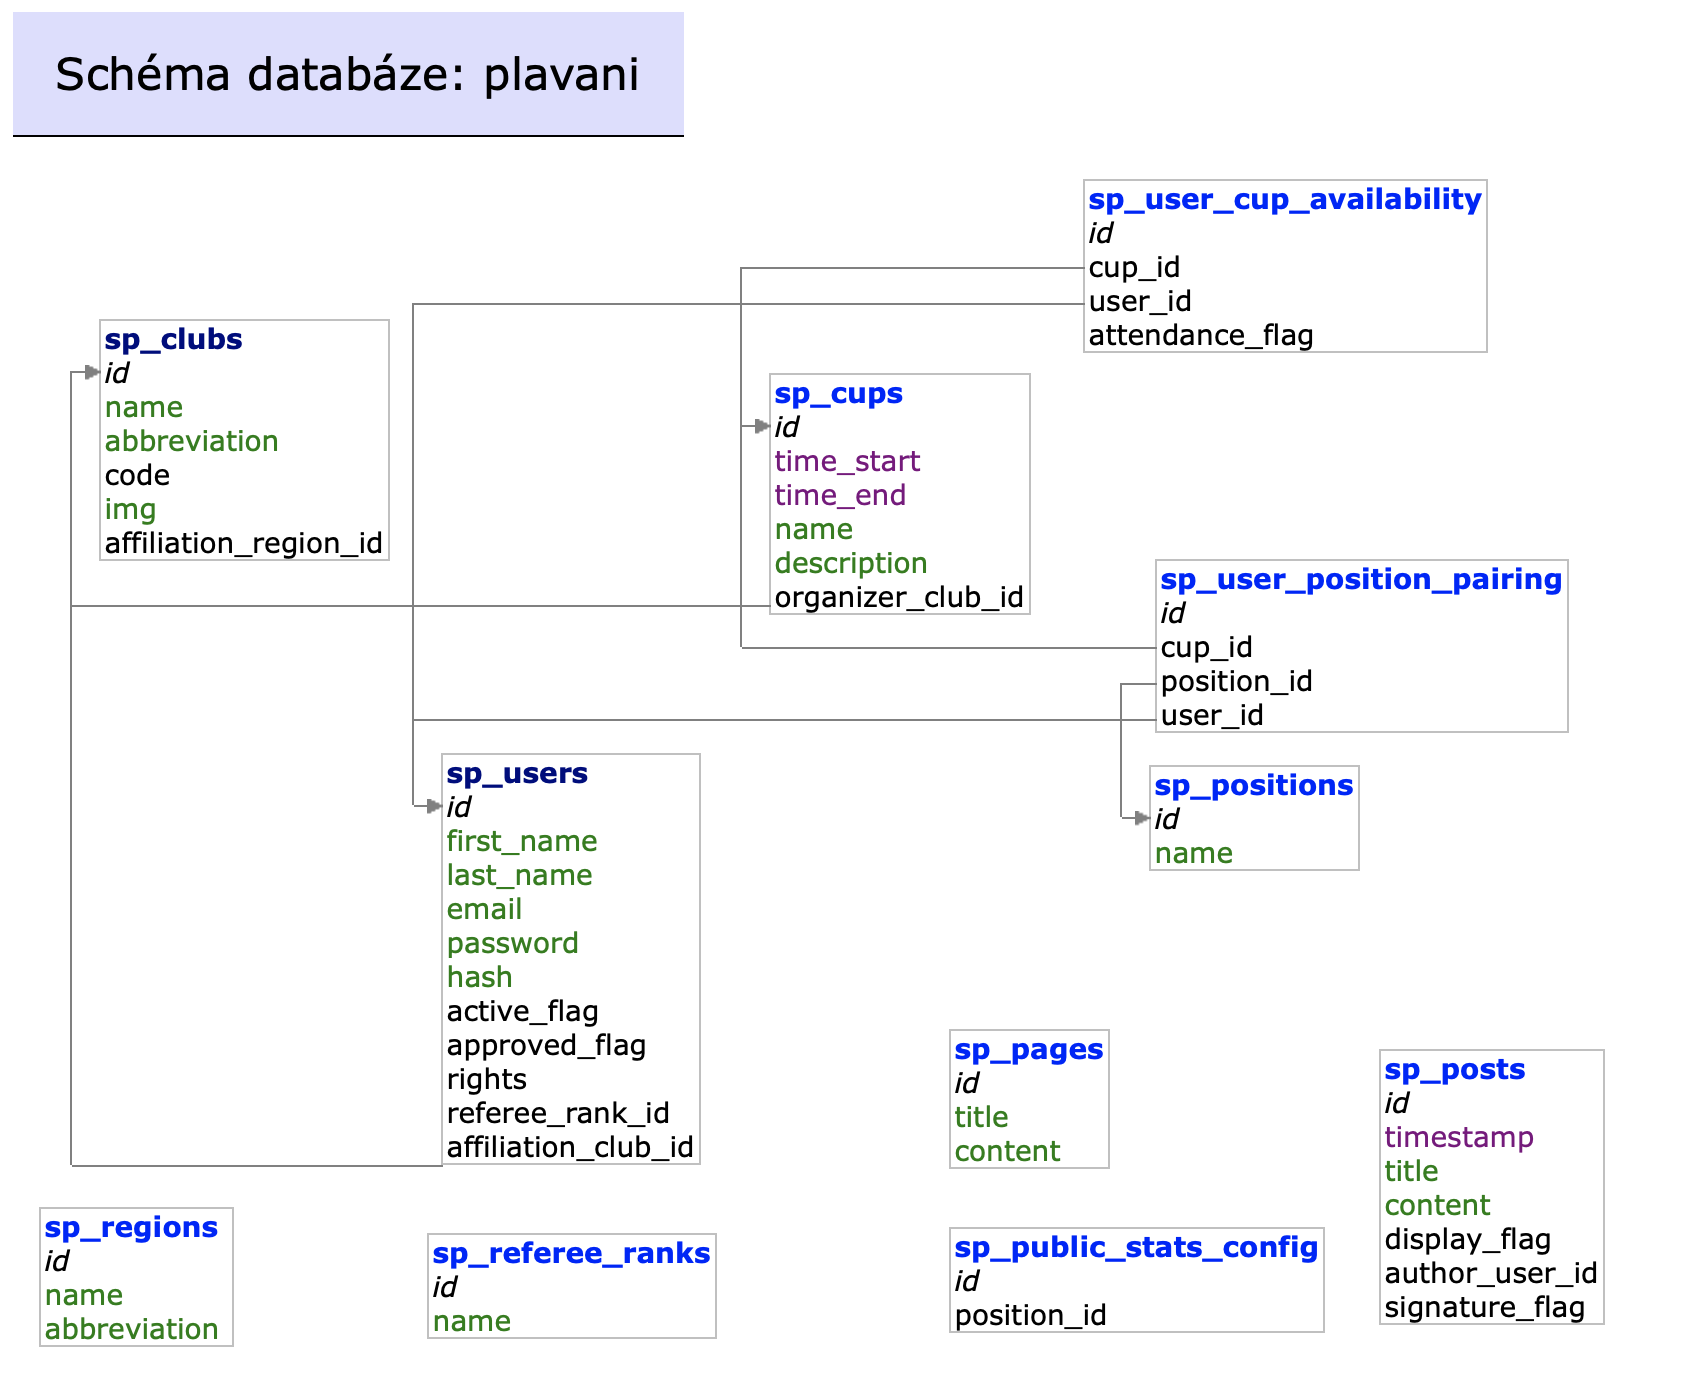
\includegraphics[scale=0.45]{imgs/schema}
\subsection{Object tables}
These are the tables in database modeling the object to satisfy the pripary motivation defined as a problem paradigm. These rows are then being converted to objects and returned to user by an apporpiate manager.
\subsubsection*{sp\_posts}
Posts for main page are stored in this table.
\newline
\underline{Table preview}
\begin{center}
  \begin{tabular}{||c c c c c c c||} 
  \hline
  id & timestamp & title & content & display\_flag & author & sign\_flag  \\ [0.5ex] 
  \hline\hline
  1 & ... & ... & ... & ... & ... & ... \\ 
  \hline
  2 & ... & ... & ... & ... & ... & ... \\ 
 \hline
  ... & ... & ... & ... & ... & ...  & ... \\ [1ex] 
  \hline
  \end{tabular}
\end{center}
\underline{Columns description}
\begin{enumerate}
  \setlength\itemsep{0em}
  \item \textbf{id}, PK, int(11), AUTOINCREMENT
  \item \textbf{timestamp}, datetime
  \item \textbf{title}, text
  \item \textbf{content}, text
  \item \textbf{display\_flag}, tinyint
  \item \textbf{author}, FK, int(11)$|$NULL
  \item \textbf{sign\_flag}, tinyint
\end{enumerate}

\subsubsection*{sp\_users}
Model users here
\newline
\underline{Table preview}
\begin{center}
  \begin{tabular}{||c c c c c c c c c c||} 
  \hline
  id & first\_name & last\_name & email & password & hash & active & approved & rights & affil \\ [0.5ex] 
  \hline\hline
  1 & Lukáš & Kousal & lukas@swim.cz & -PASS- & -HASH- & 1 & 1 & 2 & 2 \\ 
  \hline
  ... & ... & ... & ... & ... & ... & ... & ... & ... & ... \\
  \hline
  N & ... & ... & ... & ... & ... & ... & ... & ... & ... \\ [1ex] 
  \hline
 \end{tabular}
 \end{center}
 \underline{Columns description}
 \begin{enumerate}
   \setlength\itemsep{0em}
   \item \textbf{id}, PK, int(11), AUTOINCREMENT
   \item \textbf{first\_name}, varchar(50)
   \item \textbf{last\_name}, varchar(50)
   \item \textbf{email}, varchar(100) //unique identifier
   \item \textbf{password}, varchar(100)
   \item \textbf{hash}, varchar(32)
   \item \textbf{active}, tinyint(1)
   \item \textbf{approved}, tinyint(1)
   \item \textbf{rights}, int(11)
   \item \textbf{klubaffil}, FK, int(11)
\end{enumerate}

\subsubsection*{sp\_clubs}
This is how we store clubs in the 
\newline
\underline{Table preview}
\begin{center}
 \begin{tabular}{||c c c c c||} 
 \hline
 id & name & zkratka & idklubu & img \\ [0.5ex] 
 \hline\hline
 1 & Klub plaveckých sportů Vyškov & KPSVy & 614 & null.jpg \\ 
 \hline
 ... & ... & ... & ... & ... \\ 
\hline
 14 & TJ Rožnov pod Radhoštěm & TJRo & 0 & null.jpg \\ [1ex] 
 \hline
\end{tabular}
\end{center}
\underline{Columns description}
\begin{enumerate}
  \setlength\itemsep{0em}
  \item \textbf{id}, PK , int(11), AUTOINCREMENT
  \item \textbf{name}, varchar(512)
  \item \textbf{zkratka}, text
  \item \textbf{idklubu}, int(11)
  \item \textbf{img}, text
\end{enumerate}

\subsubsection*{sp\_cups}
Tabulka se závody.
\newline
\underline{Table preview}
\begin{center}
 \begin{tabular}{||c c c c c||} 
 \hline
 id & date & name & description & owningclub  \\ [0.5ex] 
 \hline\hline
 1 & 2017-06-12 & GJW Cup I. & Nejlepsi turnaj na svete & 2 \\ 
 \hline
 ... & ... & ... & ... & ...  \\ [1ex] 
 \hline
\end{tabular}
\end{center}
\underline{Columns description}
\begin{enumerate}
  \setlength\itemsep{0em}
  \item \textbf{id}, PK , int(11), AUTOINCREMENT
  \item \textbf{date}, date
  \item \textbf{name}, text
  \item \textbf{description}, text
  \item \textbf{owningclub}, int(11)
\end{enumerate}


\subsubsection*{sp\_positions}
Tabulka obsahuje všechny pozice, na které přidělujeme rozhodčí. Seznam pozic je fixní.
\newline
\underline{Table preview}
\begin{center}
 \begin{tabular}{||c c||} 
 \hline
 id & poz  \\ [0.5ex] 
 \hline\hline
 1 & Vrchní rozhodčí \\ 
 \hline
 ... & ...  \\ 
\hline
 19 & Ostatní  \\ [1ex] 
 \hline
\end{tabular}
\end{center}
\underline{Columns description}
\begin{enumerate}
  \setlength\itemsep{0em}
  \item \textbf{id}, PK , int(11), AUTOINCREMENT
  \item \textbf{poz}, varchar(512)
\end{enumerate}

\subsection{Relations tables}
Relations tables hold the most important information stored in the SwimmPair system. Both availability for cups and pairing to positions are realised here.
\subsubsection*{sp\_cup\_user\_availability}
This table stores relationships between referees/\underline{users} and \underline{cups} called availability. Referees are signed up by their team manager or themselves as available for the cup. In case of sudden inability to participate, the attendance\_flag is switched to 0 in case the user is already assigned to some position. In that case the administrator is going to see the user in red box.
\newline
\underline{Table preview}
\begin{center}
 \begin{tabular}{||c c c c||} 
 \hline
 id & cup\_id & user\_id & attendance\_flag  \\ [0.5ex] 
 \hline\hline
 1 & 3 & 21 & 1 \\ 
 \hline
 2 & 3 & 1 & 1 \\ 
 \hline
 7 & 3 & 19 & 0 \\ 
 \hline
 ... & ... & ... & ...  \\ [1ex] 
 \hline
\end{tabular}
\end{center}
\underline{Columns description}
\begin{enumerate}
  \setlength\itemsep{0em}
  \item \textbf{id}, PK, int(11), AUTOINCREMENT
  \item \textbf{cup\_id}, FK, int(11)
  \item \textbf{user\_id}, int(11)
  \item \textbf{attendance\_flag}, tinyint(1)
\end{enumerate}

\subsubsection*{sp\_position\_user\_pairing}
This table stores pairing information about available referees/users on positions for each cup. This is the most time saving utility of the SwimmPair.
\newline
\underline{Table preview}
\begin{center}
 \begin{tabular}{||c c c c||} 
 \hline
 id & cup\_id & position\_id & user\_id  \\ [0.5ex] 
 \hline\hline
 46 & 5 & 5 & 21 \\ 
 \hline
 484 & 3 & 1 & 21 \\ 
 \hline
 485 & 3 & 1 & 22 \\ 
 \hline
 486 & 3 & 2 & 7 \\
 \hline
 487 & 3 & 3 & 15 \\
 \hline
 487 & 3 & 5 & 12 \\
 \hline
 487 & 3 & 7 & 14 \\
 \hline
 ... & ... & ... & ... \\ [1ex] 
 \hline
\end{tabular}
\end{center}
\underline{Columns description}
\begin{enumerate}
  \setlength\itemsep{0em}
  \item \textbf{id}, PK, bigint(11), AUTOINCREMENT
  \item \textbf{cup\_id}, FK, int(11)
  \item \textbf{position\_id}, FK, int(11)
  \item \textbf{user\_id}, FK, int(11)
\end{enumerate}
\subsection{Content adjustment tables}
Stats positions
Pages

\section{Controllers documentation}
\par These five controllers work with objects and provide some login (i.e. joining more tables in varios ways)
\subsection{PostsManager.php}
\begin{itemize}
  \setlength\itemsep{0em}
  \item \underline{Post} $\vert$ null $\leftarrow$ \textbf{GetPostById}(\$id) $\searrow$ \_CreatePostOrNullFromStatement(\$stmt) $\searrow$ \_CreatePostFromRow(\$row)
  \item \underline{Post[]} $\vert$ null $\leftarrow$ \textbf{GetLastThreePosts}() $\searrow$ \_CreatePostsFromStatement() $\searrow$ \_CreatePostFromRow(\$row)
  \item \underline{Post[]} $\vert$ null $\leftarrow$ \textbf{GetLastNPosts}(\$N) $\searrow$ \_CreatePostsFromStatement() $\searrow$ \_CreatePostFromRow(\$row)
  \item \underline{true} $\vert$ false $\leftarrow$ \textbf{AddNewPost}(\$title, \$content)
  \item \underline{Post[]} $\vert$ false $\leftarrow$ \textbf{FindAllPostsOrderedByIdDesc}() $\searrow$ \_CreatePostsFromStatement(\$stmt) $\searrow$ \_CreatePostFromRow(\$row)
  \item \underline{true} $\vert$ false $\leftarrow$ \textbf{UpdatePost}(\$id, \$title, \$article)
\end{itemize}
\subsection{UsersManager.php}
\begin{itemize}
  \setlength\itemsep{0em}
  \item \underline{User} $\vert$ null $\leftarrow$ \textbf{GetUserById}(\$id) $\searrow$ \_CreateUserOrNullFromStatement(\$stmt) $\searrow$ \_CreateUserFromRow(\$row)
  \item \underline{User[]} $\vert$ null $\leftarrow$ \textbf{FindAllActiveUsersOrderByLastNameDesc} $\searrow$ \_CreateUsersFromStatement(\$stmt) $\hookrightarrow$ \_CreateUserFromRow (\$row)
  \item \underline{User[]} $\vert$ null $\leftarrow$ \textbf{FindAllInactiveUsersOrderByLastNameDesc} $\searrow$ \_CreateUsersFromStatement(\$stmt) $\hookrightarrow$ \_CreateUserFromRow (\$row)
  \item \underline{User[]} $\vert$ null $\leftarrow$ \textbf{FindAllRegisteredComradesForTheCup}(\$cupID, \$teamID) $\searrow$ \_CreateUsersFromStatement(\$stmt) $\hookrightarrow$ \_CreateUserFromRow (\$row)
  \item \underline{User[]} $\vert$ null $\leftarrow$ \textbf{FindAllComrades}(\$teamID) $\searrow$ \_CreateUsersFromStatement(\$stmt) $\hookrightarrow$ \_CreateUserFromRow(\$row)
  \item \underline{User[]} $\vert$ null $\leftarrow$ \textbf{FindAllRegisteredUsersForTheCup}(\$cupID) $\searrow$ \_CreateUsersFromStatement(\$stmt) $\hookrightarrow$ \_CreateUserFromRow(\$row)
  \item \underline{User[]} $\vert$ null $\leftarrow$ \textbf{FindAllNametagsForTheCup}(\$cupID) $\searrow$ \_CreateUsersFromStatement(\$stmt) $\hookrightarrow$ \_CreateUserFromRow(\$row)
  \item \underline{User[]} $\vert$ null $\leftarrow$ \textbf{FindPairedUsersOnCupForPosition}(\$cupID, \$posID) $\searrow$ \_CreateUsersFromStatement(\$stmt) $\hookrightarrow$ \_CreateUserFromRow(\$row)
  \item \underline{Pair[]} $\vert$ null $\leftarrow$ \textbf{FindPairedPozIDUserIDOnCup}(\$cupID) $\searrow$ \_CreatePairsFromStatement(\$stmt) $\hookrightarrow$ \_CreatePairFromRow(\$row)
  \item \underline{string} $\vert$ null $\leftarrow$ \textbf{GetClubAbbreviationByAffiliationId}(\$id) $\searrow$ \_GetSingleResultFromStatement(\$stmt)
  \item \underline{string} $\vert$ null $\leftarrow$ \textbf{GetUserFullNameById}(\$id) $\searrow$ \_GetSingleResultFromTwoColsStatement(\$stmt)
  \item \underline{true} $\vert$ \underline{false} $\leftarrow$ \textbf{UserWithEmailExists}(\$email)
  \item \underline{true} $\vert$ false $\leftarrow$ \textbf{RegisterUserFromAdmin}(\$first\_name, \$last\_name, \$email, \$password, \$rights, \$klubaffil)
  \item \underline{true} $\vert$ false $\leftarrow$ \textbf{SendYouWereRegisteredFromAdmin}(\$email, \$password)
  \item \underline{true} $\vert$ false $\leftarrow$ \textbf{ApproveUser}(\$userID)
  \item \underline{true} $\vert$ false $\leftarrow$ \textbf{UpdatePairing}(\$JSON) //TBReimplemented in controller
  \item \underline{true} $\vert$ false $\leftarrow$ \textbf{RegisterUserFromAdminWrap}(\$first\_name, \$last\_name, \$email, \$password, \$prava, \$klub) check, register if possible ($\searrow$ true(not registering) | \underline{false} $\leftarrow$ userWithEmailExists(\$email) | $\searrow$ registerUserFromAdmin(\$first\_name, \$last\_name, \$email, \$password, \$prava, \$klub))
  \item \underline{token(Action::SUCC, -creds-)} $\vert$ token(Action::UNFOUND, -null-) | token(Action::WRONGCRED, -null-) $\leftarrow$ \textbf{loginFromXamarin}(\$username, \$password)
\end{itemize}
\subsection{ClubsManager.php}
\begin{itemize}
  \setlength\itemsep{0em}
  \item \underline{Club} | null $\leftarrow$ \textbf{GetClubById}(\$id) $\searrow$ \_CreateClubFromStatement(\$stmt) $\searrow$ \_CreateClubFromRow(\$row)
  \item \underline{Club []} | null $\leftarrow$ \textbf{FindAllClubs}() $\searrow$ \_CreateClubsFromStatement(\$stmt) $\hookrightarrow$ \_CsreateClubFromRow(\$row)
\end{itemize}
\subsection{CupsManager.php}
\begin{itemize}
  \setlength\itemsep{0em}
  \item \underline{Cup[]} $\vert$ null $\leftarrow$ \textbf{FindAllUpcomingCupsEarliestFirst}() $\searrow$ \_CreateCupsFromStatement(\$stmt) $\hookrightarrow$ \_CreateCupFromRow(\$row)
  \item \underline{Cup[]} $\vert$ null $\leftarrow$ \textbf{FindAllPastCupsMostRecentFirst}() $\searrow$ \_CreateCupsFromStatement(\$stmt) $\hookrightarrow$ \_CreateCupFromRow(\$row)
  \item \underline{string} $\vert$ null  $\leftarrow$ \textbf{GetCupNameById}(\$id) $\searrow$ \_GetSingleResultFromStatement(\$stmt) $\searrow$ \_GetSingleResultFromStatement (\$stmt)
  \item \underline{Cup} $\vert$ null  $\leftarrow$  \textbf{GetCupById}(\$id) $\searrow$ \_CreateCupOrNullFromStatement(\$stmt)  $\searrow$ \_CreateCupFromRow(\$row)
  \item \underline{Pair[]} $\vert$ null $\leftarrow$  \textbf{FindPairingsForThisCup}(\$id) $\searrow$ \_CreatePairsFromStatement(\$stmt) $\hookrightarrow$ \_CreatePairFromRow(\$row)
  \item \underline{true} $\vert$ false $\leftarrow$  \textbf{InsertNewCupFromAdmin}(\$name, \$date, \$club, \$content)
  \item \underline{true} $\vert$ \underline{false} $\leftarrow$  \textbf{IsUserAvailableForTheCup}(\$userID, \$cupID)
  \item \underline{true} $\vert$ false $\leftarrow$  \textbf{UpdatePairingForThisCup}(\$cupID, \$json)
  \item \underline{true} $\vert$ false $\leftarrow$  \textbf{UpdateAvailabilityForThisCup}(\$cupID, \$json)
  \item \underline{true} $\vert$ false $\leftarrow$  \textbf{AddAvailableUserForTheCup}(\$cupID, \$userID)
\end{itemize}
\subsection{PositionsManager.php}
\begin{itemize}
  \setlength\itemsep{0em}
  \item \underline{Position[]} $\vert$ null $\leftarrow$  \textbf{FindAllPositions}() $\searrow$ \_CreatePositionsFromStatement(\$stmt) $\hookrightarrow$ \_CreatePositionFromRow(\$row)
  \item \underline{string} $\vert$ null $\leftarrow$ \textbf{GetPositionNameById}(\$id) $\searrow$ \_GetSingleResultFromStatement(\$stmt)
\end{itemize}
\newpage
\section{Application structure}
\subsection*{User part of the system}
Whole system must be running on Czech URLs for convinience reasons of administrators. English equivalents are attached. 
\newline
\begin{forest}
  for tree={
    font=\ttfamily,
    grow'=0,
    child anchor=west,
    parent anchor=south,
    anchor=west,
    calign=first,
    edge path={
      \noexpand\path [draw, \forestoption{edge}]
      (!u.south west) +(7.5pt,0) |- node[fill,inner sep=1.25pt] {} (.child anchor)\forestoption{edge label};
    },
    before typesetting nodes={
      if n=1
        {insert before={[,phantom]}}
        {}
    },
    fit=band,
    before computing xy={l=15pt},
  }
[SwimmPair
  [index.php]
  [Zavody (Cups)
    [nadchazejici.php (upcoming.php)
      [zavod.php (cup.php)]
    ]
    [archiv.php (archive.php)
      [zavod.php (cup.php)] 
    ]
  ]
  [Rozhodci (Referees)
    [lide.php (users.php)
      [clovek.php (user.php)]
    ]
    [kluby.php (clubs.php)
      [klub.php (club.php)]
    ]
  ]
  [/pravidla/index.php (/rules/index.php)]
  [kontakty.php (contacts.php)]
  [/admin/index.php]
]
\end{forest}
\newpage
\subsection*{Administrative part of the system} 
The administration has following structure. Regarding yor rights have following structure. Each user has profile settings for reseting password and other stuff.  
\newline
\begin{forest}
  for tree={
    font=\ttfamily,
    grow'=0,
    child anchor=west,
    parent anchor=south,
    anchor=west,
    calign=first,
    edge path={
      \noexpand\path [draw, \forestoption{edge}]
      (!u.south west) +(7.5pt,0) |- node[fill,inner sep=1.25pt] {} (.child anchor)\forestoption{edge label};
    },
    before typesetting nodes={
      if n=1
        {insert before={[,phantom]}}
        {}
    },
    fit=band,
    before computing xy={l=15pt},
  }
[Administration
  [pridat\_aktualitu.php (add\_post.php)]
  [editovat\_aktuality.php (edit\_posts.php)
    [editovat\_aktualitu.php (edit\_post.php)]
  ]
  [nove\_registrovani.php (newly\_registered.php)]
  [rozhodci\_zavody.php (referees\_cups.php)
    [pairing.php (pairing.php)]
  ]
  [zaregistrovat\_uzivatele.php (register\_user.php)]
  [editovat\_profily.php (edit\_profiles.php)
    [editovat\_profil.php (edit\_profile.php)]
  ]
  [novy\_klub.php (add\_club.php)]
  [sprava\_klubu.php (edit\_clubs.php)
    [editovat\_klub.php (edit\_club.php)]
  ]
  [novy\_kraj.php (new\_region.php)]
  [sprava\_kraju.php (edit\_regions.php)
    [editovat\_kraj.php (edit\_region.php)]
  ]
  [konfigurace\_statistik.php (configure\_stats.php)]
  [editovat\_stranku.php (edit\_page.php)]
]
\end{forest}
\newline
\begin{forest}
  for tree={
    font=\ttfamily,
    grow'=0,
    child anchor=west,
    parent anchor=south,
    anchor=west,
    calign=first,
    edge path={
      \noexpand\path [draw, \forestoption{edge}]
      (!u.south west) +(7.5pt,0) |- node[fill,inner sep=1.25pt] {} (.child anchor)\forestoption{edge label};
    },
    before typesetting nodes={
      if n=1
        {insert before={[,phantom]}}
        {}
    },
    fit=band,
    before computing xy={l=15pt},
  }
[My Club
  [pridat\_zavod.php (add\_cup.php)]
  [prihlasit\_moje\_lidi.php (sign\_availability\_mates.php)
    [prihlasit\_moje\_lidi\_na.php (sign\_availability\_mates\_for.php)]
  ]
]
\end{forest}
\newline
\begin{forest}
  for tree={
    font=\ttfamily,
    grow'=0,
    child anchor=west,
    parent anchor=south,
    anchor=west,
    calign=first,
    edge path={
      \noexpand\path [draw, \forestoption{edge}]
      (!u.south west) +(7.5pt,0) |- node[fill,inner sep=1.25pt] {} (.child anchor)\forestoption{edge label};
    },
    before typesetting nodes={
      if n=1
        {insert before={[,phantom]}}
        {}
    },
    fit=band,
    before computing xy={l=15pt},
  }
[Me
  [sebe\_na\_zavod.php (myself\_for\_cup.php)
    [prihlasit\_se\_na.php (sign\_myself\_for.php)]
  ]
]
\end{forest}
\newline
\section{JavaScript functions documentation}
Several cool features for the web to make it more useful are described here.
\subsection*{XMLHttpRequest/}
\begin{itemize}
    \item getarticleid.php, \textbf{GET args}: id
    \item getpersonstatisticsfortheseason.php, \textbf{GET args}: user\textunderscore id, year
    \item getclubstatisticsfortheseason.php, \textbf{GET args}: club\textunderscore id, year
\end{itemize}
\subsection{Previous post}
This button on the main page serves as a tool for loading next post. This button has onclick="GetPostAppendPost(PushLastID())". These are both JavaScript functions, PushLastID() detects id "I" of last post from DOM by query and returns it. This value is then used as an argument of call GetPostAppendPost(I). This function requests article by opening GET request XMLHttpRequest/getarticleid?id="I". If result is null, button is deleted since there are no other articles to pull from DB. Otherwise next article is constructed.
\subsection{Personal statistics change year}
All individual referees have season picker when opened. Default season is this season. Clicking different season visibily changes selected year and obtains statistics and updates the table. Clicking onclick="processPersonForTheSeason(user-id, updatePairingForThisCup)" calls communicateStatsXHRAndPopulateStats(user-id, year) which gets data from XMLHttpRequest/getpersonstatisticsfortheseason. 
\subsection{Club statistics change year}
Club statistics are updated by clicking appropriate year, which gets visibly switched. Year onclick calls processClubForTheSeason(club-id, this) which gets statistics by calling communicateClubStatisticsXMHAndPopulateTable(club-id, year) which gets data by calling XMLHttpRequest/getclubstatisticsfortheseason and subsequently calling refreshClubStatsInTheTable(returnedGetJSON) which literally puts the stats in.
\subsection{Filtering referees}
This function is triggered by one of these: KrajPickerTapped(this), TridaPickerTapped(this) or SearchPerformed(). Each one calls FilterRozhodci("kraje", "tridy", "inputTrida", "nopplfound"). We then loop all people visible/hidden and check if this one's Region IsPermissible(args[]), then if one's Class IsPermissible(args[]) and then if one's IsNamePermissible(args[]). We then set one element style to style="" and continue cycle execution. If we fail one of these three conditions we proceed to code below which sets element style to style="display:none". After the cycle when check the aux variable and if our query is indeed empty we write it for the user.
\par
This long procedure gets triggered and subsequently executed everytime region, class or name is changed. Performance should be fine here since the algorithm is dependent on human input. 

\section{SwimmPair REST API}

\section{Mobile app structure}
Phone version of our administration follows the same structure. All objects are same, including data type, which have to be explicitly defined, unline in PHP.
